\documentclass{article}
\usepackage[utf8]{inputenc}
\usepackage[margin=1in]{geometry}
\usepackage{amsmath}
\usepackage{graphicx}
\graphicspath{{plots/}}
\setlength{\parindent}{0em}
\setlength{\parskip}{0.5em}

\title{CTA200 Assignment 2}
\author{Emily Crawley}
\date{05/05/2021}

\begin{document}

\maketitle

\section*{Question 1}

Using the approximation given for evaluating a function $f(x)$ at $x_0$ for small finite $h$, we define \texttt{deriv(f, x0, h)} which computes

$$ \frac{f(x_0 + h) - f(x_0 - h)}{2h} $$

We then define our function to be differentiated, \texttt{f(x) = sin(x)} and its analytical derivative \texttt{dfdx(x) = cos(x)}. Values of $h < 1$ were chosen ranging from 0.1 to 1e-8.

We compute the analytical derivative $cos(0.1)$, and the numerical derivatives at each value of $h$, plotting them each against the analytical solution. Since the $h$ values vary by orders of 10 we plot the error on logarithmic axes using \texttt{pyplot.loglog}.

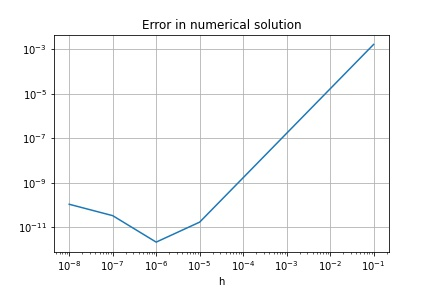
\includegraphics[scale=0.7]{plot1}

From the plot we can see that the error in the numerical solution decreases linearly for smaller values of $h$, until around $h < 10^{-6}$ when the larger relative error presumably comes from the precision limitations of the \texttt{float} type. The slope of the linear part of the graph represents how quickly the error decreases as $h$ decreases, so in some sense represents its effectiveness in terms of accuracy. That is, we want to be able to greatly decrease error with only one or two order-of-magnitude decrements of $h$, so a steeper slope is preferable.

\section*{Question 2}

We cover the complex plane in the square $|z|^2 = \Re(z)^2 + \Im(z)^2$ by taking $c = x + iy$ for numerous combinations of x- and y-values between -2 and 2.

For each point $c$ we iterate the expression $z_{i + 1} = z_i^2 + c$ starting from $z_0 = 0$ and test the absolute square of each $z_i$ to see if it diverges from the boundary. If so, we assign it a value of 0 in a 2D boolean array representing whether each point is bounded or not. We also record the iteration number in a separate 2D array. The iteration number array contains values of -1 for points that stay bounded. We then plot the results using \texttt{pyplot.imshow}.

When tested running for 1000 iterations, none of the points in the sample set take more than 32 iterations to diverge, so to save time we will only iterate for 32 steps.

The only obvious pattern from the resulting images is that there are no points that remain bounded from our iteration in an area centered around $c = -0.5i$. This same area on the iteration numbers plot also notably contains the brightest points, i.e. the points in these areas take a higher number of iterations to diverge. There is a single point near the center of this area that notably takes the single highest number of iterations to diverge. These results are taken from a finite number of points across the area and not every possible point, so there could be more "interesting" points that are missed by numerical analysis.

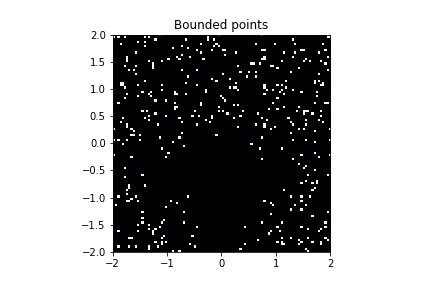
\includegraphics[scale=0.7]{plot2_1}

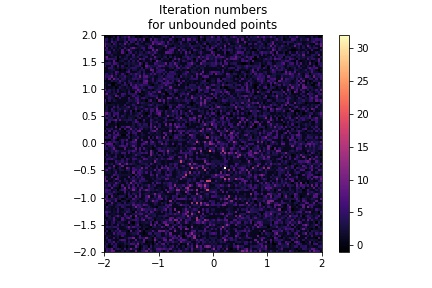
\includegraphics[scale=0.7]{plot2_2}

\section*{Question 3}

Our initial value problem is given as:

\begin{align}
    \frac{dS}{dt} &= -\frac{\beta S I}{N},\\
    \frac{dI}{dt} &= \frac{\beta S I}{N} - \gamma I,\\
    \frac{dR}{dt} &= \gamma I
\end{align}

$I(0) = 1, S(0)=999, R(0) = 0$

$N=1000$, $0\leq t \leq 200$

Using \texttt{scipy.integrate.solve\_ivp} as the ODE integrator, which takes parameters \texttt{(fun, tspan, y0)}, we set up the time derivative functions as a vector $[\frac{dS}{dt},\frac{dI}{dt},\frac{dR}{dt}]$ for the \texttt{fun} parameter, and the initial conditions vector $[S(0), I(0), R(0)]$ as \texttt{y0}. We also specify the parameter \texttt{vectorized=True} so that the integrator handles the vectors properly. We will use its default Runge-Kutta method, \texttt{method='RK45'}.

$\beta$ represents an infection rate and $\gamma$ represents a recovery rate, so we will select some meaningful variations on these parameters, i.e. a disease that spreads quickly but has a fast recovery rate, a disease that spreads quickly with a slower recovery rate, etc. The solutions show us the different progressions for each of these sets of parameters, for example with a high infection rate and low recovery rate there is a large spike in $I(t)$, whereas with the same infection rate but a higher recovery rate the $I(t)$ "spike" is much lower as the disease does not have the opportunity to progress. The first three scenarios plotted all have the recovered and susceptible populations become constant when the infected population reaches zero. With a zero recovery rate, the entire population eventually becomes infected.

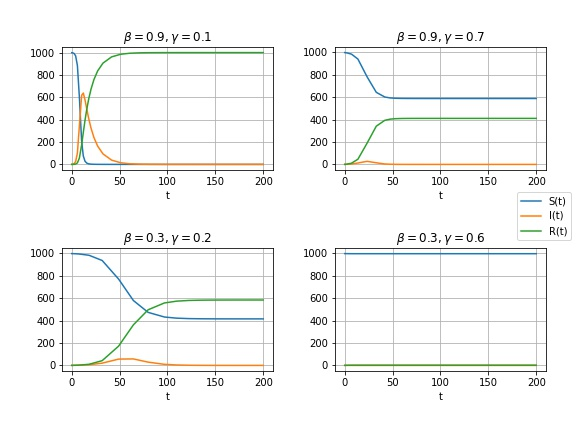
\includegraphics[scale=0.7]{plot3}

\end{document}